\section{The distance that remains}\label{sec:distance}

This section reports IC/rho, with greater than 1 meaning rho is cheaper. It
gives the current figure for each family, the reference it uses, and how
that figure moved over the period.

\begin{figure}[t]
\centering
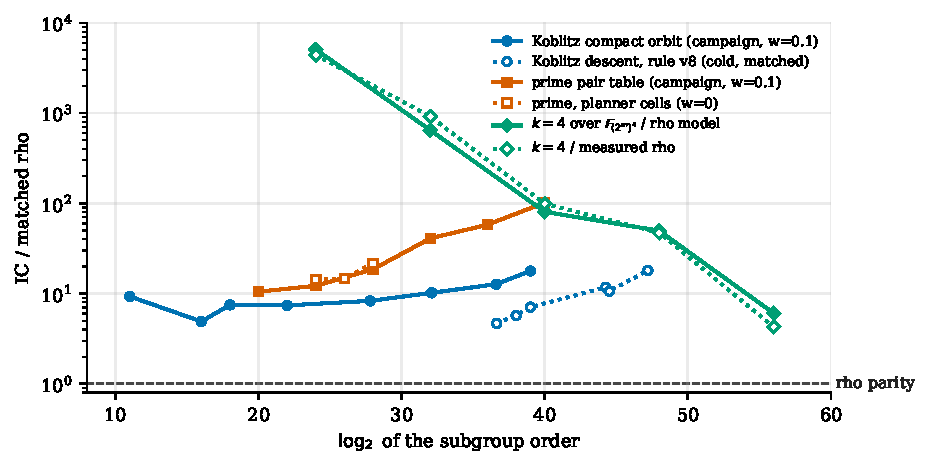
\includegraphics[width=\linewidth]{figures/fig-families.pdf}
\caption[]{Distance to matched rho by family and size. Koblitz and prime
curves use the frontier campaign's priced arms ($w=0.1$, 16 targets
$\times$ 2 rounds) and, open markers, the Koblitz rule at v8 (cold, 64
targets) and the prime planner cells ($w=0$). $k=4$ over $\FF_{(2^m)^4}$
uses the char-2 ladder against the negation-map rho model (filled) and a
measured rho (open); the $n\approx2^{56}$ point is one target. Curves and
units differ between families, so the lines are not ranked against each
other. Sources: \art{figures/data.json}.}
\label{fig:families}
\end{figure}

\subsection{Koblitz curves: the rule at a matched rho}

The leaderboard's Table~A measures a Koblitz descent (aimed $m=3$
collection, $m=2$ or $m=3$ descent) cold on one unseen public point per
process: 64 points per size and six sizes from $2^{36.6}$ to $2^{47.2}$.
It was re-run three times on the same instances
(\art{research/ic_tool_program/rule/}), and Figure~\ref{fig:koblitz} shows
all three.
\begin{itemize}
\item \emph{v3 to v7: an IC improvement.} With the same rho, IC became
  $1.52$--$1.89\times$ faster (\#1978), and the cold ratio fell from
  $5.23$--$20.97$ to $3.43$--$11.51$.
\item \emph{v8: a matched reference.} The rule was run on one binary with
  rho's signed-Frobenius canonicalisation batched 16 lanes wide, against a
  same-binary control with rho as at v7. In both runs 408 of 408 rows pass
  the \texttt{vs\_rho} check, and the matched rho takes the same walks as
  the control on 64 of 64 targets per size. IC's online time is unchanged
  between runs ($0.976$--$1.033$). Rho's online time fell $1.42$--$1.62\times$.
  The cold gap against the matched rho is
  \[
    4.67\,[4.34,5.07],\ 5.70,\ 7.07,\ 11.75,\ 10.65,\ 18.07\,[15.98,20.58]
  \]
  at $\log_2 r=36.6, 38.0, 39.0, 44.3, 44.5, 47.2$. All six values lie
  inside ranges declared before the rows were taken
  (\art{research/ic_tool_program/rule/v8/README.md}).
\end{itemize}
Two readings follow, and both hold.
\begin{itemize}
\item The $1.52$--$1.89\times$ IC improvement is real and \cls{engineering}.
\item Against the matched rho, v8's distance sits about where v3's sat
  against the old rho. The fitted slope of the gap is $0.168$ $[0.128,0.208]$
  per $\ln r$, against v3's $0.176$. The apparent flattening between v3 and
  v7 was mostly an artefact of an unmatched rho. The class of v8 is
  \cls{engineering} on the rho side and \cls{accounting} for the gap.
\end{itemize}
Pricing rho at its canonical step instead of as built gives a model gap of
$6.45$--$23.32\times$. The validation sweep, recomputing Table~A's rows that
way, reads $9.13$--$41.13\times$
(\art{research/validation_sweep_20261019/A-leaderboard/REPORT.md}). The
leaderboard still prints the v3 ratios; the v8 figures supersede them as the
distance remaining.

\begin{figure}[t]
\centering
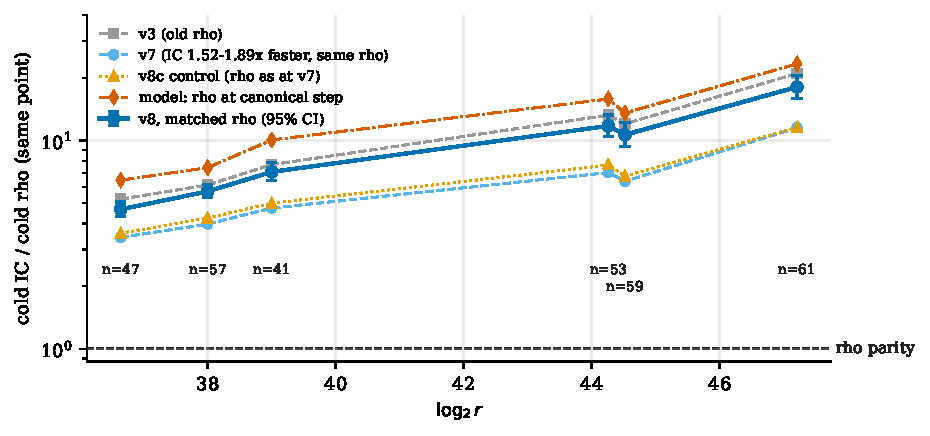
\includegraphics[width=\linewidth]{figures/fig-koblitz-rule.pdf}
\caption[]{The Koblitz rule at three baselines, cold IC over cold rho on the
same public point, 64 targets per size. v3 to v7 is an IC improvement with
the same rho; v8 is the same IC against a matched (faster) rho, with a
same-binary control (v8c) that reproduces v7. The dash-dot line prices rho
at the canonical step. Source:
\art{research/ic_tool_program/rule/v8/README.md}.}
\label{fig:koblitz}
\end{figure}

\paragraph{The priced campaign.} The frontier campaign
(\art{research/ic_frontier_campaign_20261015/}) ran every method family on
the same fixed ladders, with 16 public targets per curve and every native
operation priced across the band. Of its 4{,}848 executions, 3{,}178
measured runs were verified, and 19 of 19 replay audits were identical. The
closest Koblitz arm, compact orbit, is $3.8$--$15\times$ signed-Frobenius
rho at $w=0$ and $4.9$--$17.8\times$ at $w=0.1$. Its fitted exponent on
$n=37$--$47$ is $0.589$ $[0.518,0.743]$, against rho's $0.436$
$[0.358,0.508]$, separated at $w=0$ only.

\paragraph{$n=83$.} The last cold measurement is the 16 October holdout
with K1120, on five public points: IC at $119.826$\,s cold against
rho's mean $2.164$\,s on the same points, a ratio of
$55.368$ (\art{research/n83_e2e_holdout_20261016/RESULT.md}). Its frozen
selection is \texttt{BOUNDED\_UNKNOWN}. K1107 since cut $1.195$\,s from a
$115$\,s process (\S\ref{sec:basis}), which moves this ratio by about 1\%.
The stacked producer's in-run gap of $94.4$ uses a different baseline and
rho measurement (\S\ref{sec:setup}). Two $n=83$ baselines in the
\texttt{crypto} and \texttt{cryptanalysis} repositories ($120$\,s and
$195.7$\,s) are not yet reconciled.

\subsection{Prime curves}

\begin{itemize}
\item \emph{Campaign.} The two-summand pair-table arm goes from $10.5\times$
  rho with negation at 20 bits to $101.8\times$ at 40 bits ($w=0.1$). Its
  fitted exponent is $0.620$ $[0.557,0.663]$, against rho's $0.435$, which
  is the $r^{2/3}$ against $r^{1/2}$ of \S\ref{sec:model}. The Kummer-tower
  arm is $28$--$159\times$.
\item \emph{Planner.} A cost-model planner chose the base and arity per
  curve, and was validated on six registered and three supplementary prime
  curves. The plan beats every alternative arm at $w=0$, and rho is
  cheaper on every curve, by $12.6$--$25.8\times$. The best registered cell
  is $14.39$ $[11.63,18.45]$ at 24 bits, against a predicted $12.23$
  (1{,}152 runs, all verified, 72 exact replays;
  \art{research/ic_planner_validation_20261020/README.md}).
\item \emph{ECCp-131.} Exact relation paths were built for the Certicom
  ECCp-131 parameters, as a correctness exercise. Every arm found zero
  relations: a two-sum probe at $B=512$ and a three-point probe whose hit
  probability is at most $2^{-106.19}$ at $B=128$. The 20-bit ecbench
  control on the same code path, a different curve, is $9.41$
  $[7.22,12.93]\times$ rho
  (\art{research/eccp131_bsgs_ic_20261020/REPORT.md}).
\end{itemize}

\subsection{Nearest approaches}

Table~\ref{tab:nearest} collects the smallest IC/rho the programme has
measured, with the qualifier each one carries. No entry is below 1 on an
elliptic curve with a matched cold reference.

\begin{table}[t]
\centering\small
\caption[]{Smallest measured distances to rho, by family.}
\label{tab:nearest}
\begin{tabularx}{\linewidth}{@{}>{\raggedright}p{3.6cm}l>{\raggedright\arraybackslash}X@{}}
\toprule
Family & IC/rho & Qualifier \\
\midrule
Genus 3 via cubic GHS, $q=2^{20}$ & $1.15$ & measured negation rho; overlapping, not identical curves; two later rounds ($0.44\times$) unmatched \\
$k=4$, $\FF_{(2^m)^4}$, $m=14$ & $4.27$ & one target; $6.06\times$ the rho model; closing as $n^{-1/4}$ \\
Koblitz, fully priced orbit & $1.566$ $[0.99,2.35]$ & best cell of a ladder; ratio never below 1; grows as $r^{0.165}$ \\
Koblitz rule v8, $2^{36.6}$ & $4.67$ $[4.34,5.07]$ & cold, matched, 64 targets \\
Prime, 20 bits & $10.5$ & campaign, $w=0.1$; $r^{1/6}$ widening \\
Prime, planner 24 bits & $14.39$ $[11.63,18.45]$ & $w=0$ \\
Koblitz $n=83$ & $55.4$ & cold, K1120, \texttt{BOUNDED\_UNKNOWN} \\
\bottomrule
\end{tabularx}
\end{table}
